\documentclass[10pt,a4paper]{article}
\usepackage[utf8]{inputenc}
\usepackage{amsmath}
\usepackage{amsfonts}
\usepackage{amssymb}
\usepackage{graphicx}
\usepackage{subfig}
\usepackage{helvet}
\usepackage[frenchb]{babel}
\usepackage[left=2.00cm, right=2.00cm, top=3.00cm, bottom=3.00cm]{geometry}
\renewcommand\familydefault{\sfdefault}
\usepackage{fancyhdr}
\pagestyle{fancy}

\usepackage[gobble=auto]{pythontex}

\title{Hackathon Workshop 2024}

\fancyhead[L]{
\includegraphics[height=1cm]{logo_CSMAJuniors.png}}
\fancyhead[C]{HACKATHON}
\fancyhead[R]{Tetris}
\author{Aurélien Grolet - Paul Oumaziz}

\usepackage{amsthm}
\usepackage{thmtools}
\usepackage{tcolorbox}
\usepackage{minted}

\tcbuselibrary{minted,skins}
\setminted[python]{breaklines, framesep=2mm, numbersep=5pt,tabsize=4}

\definecolor{bg}{rgb}{0.95,0.95,0.95}

\begin{document}

\begin{figure}[ht!]
	\centering
	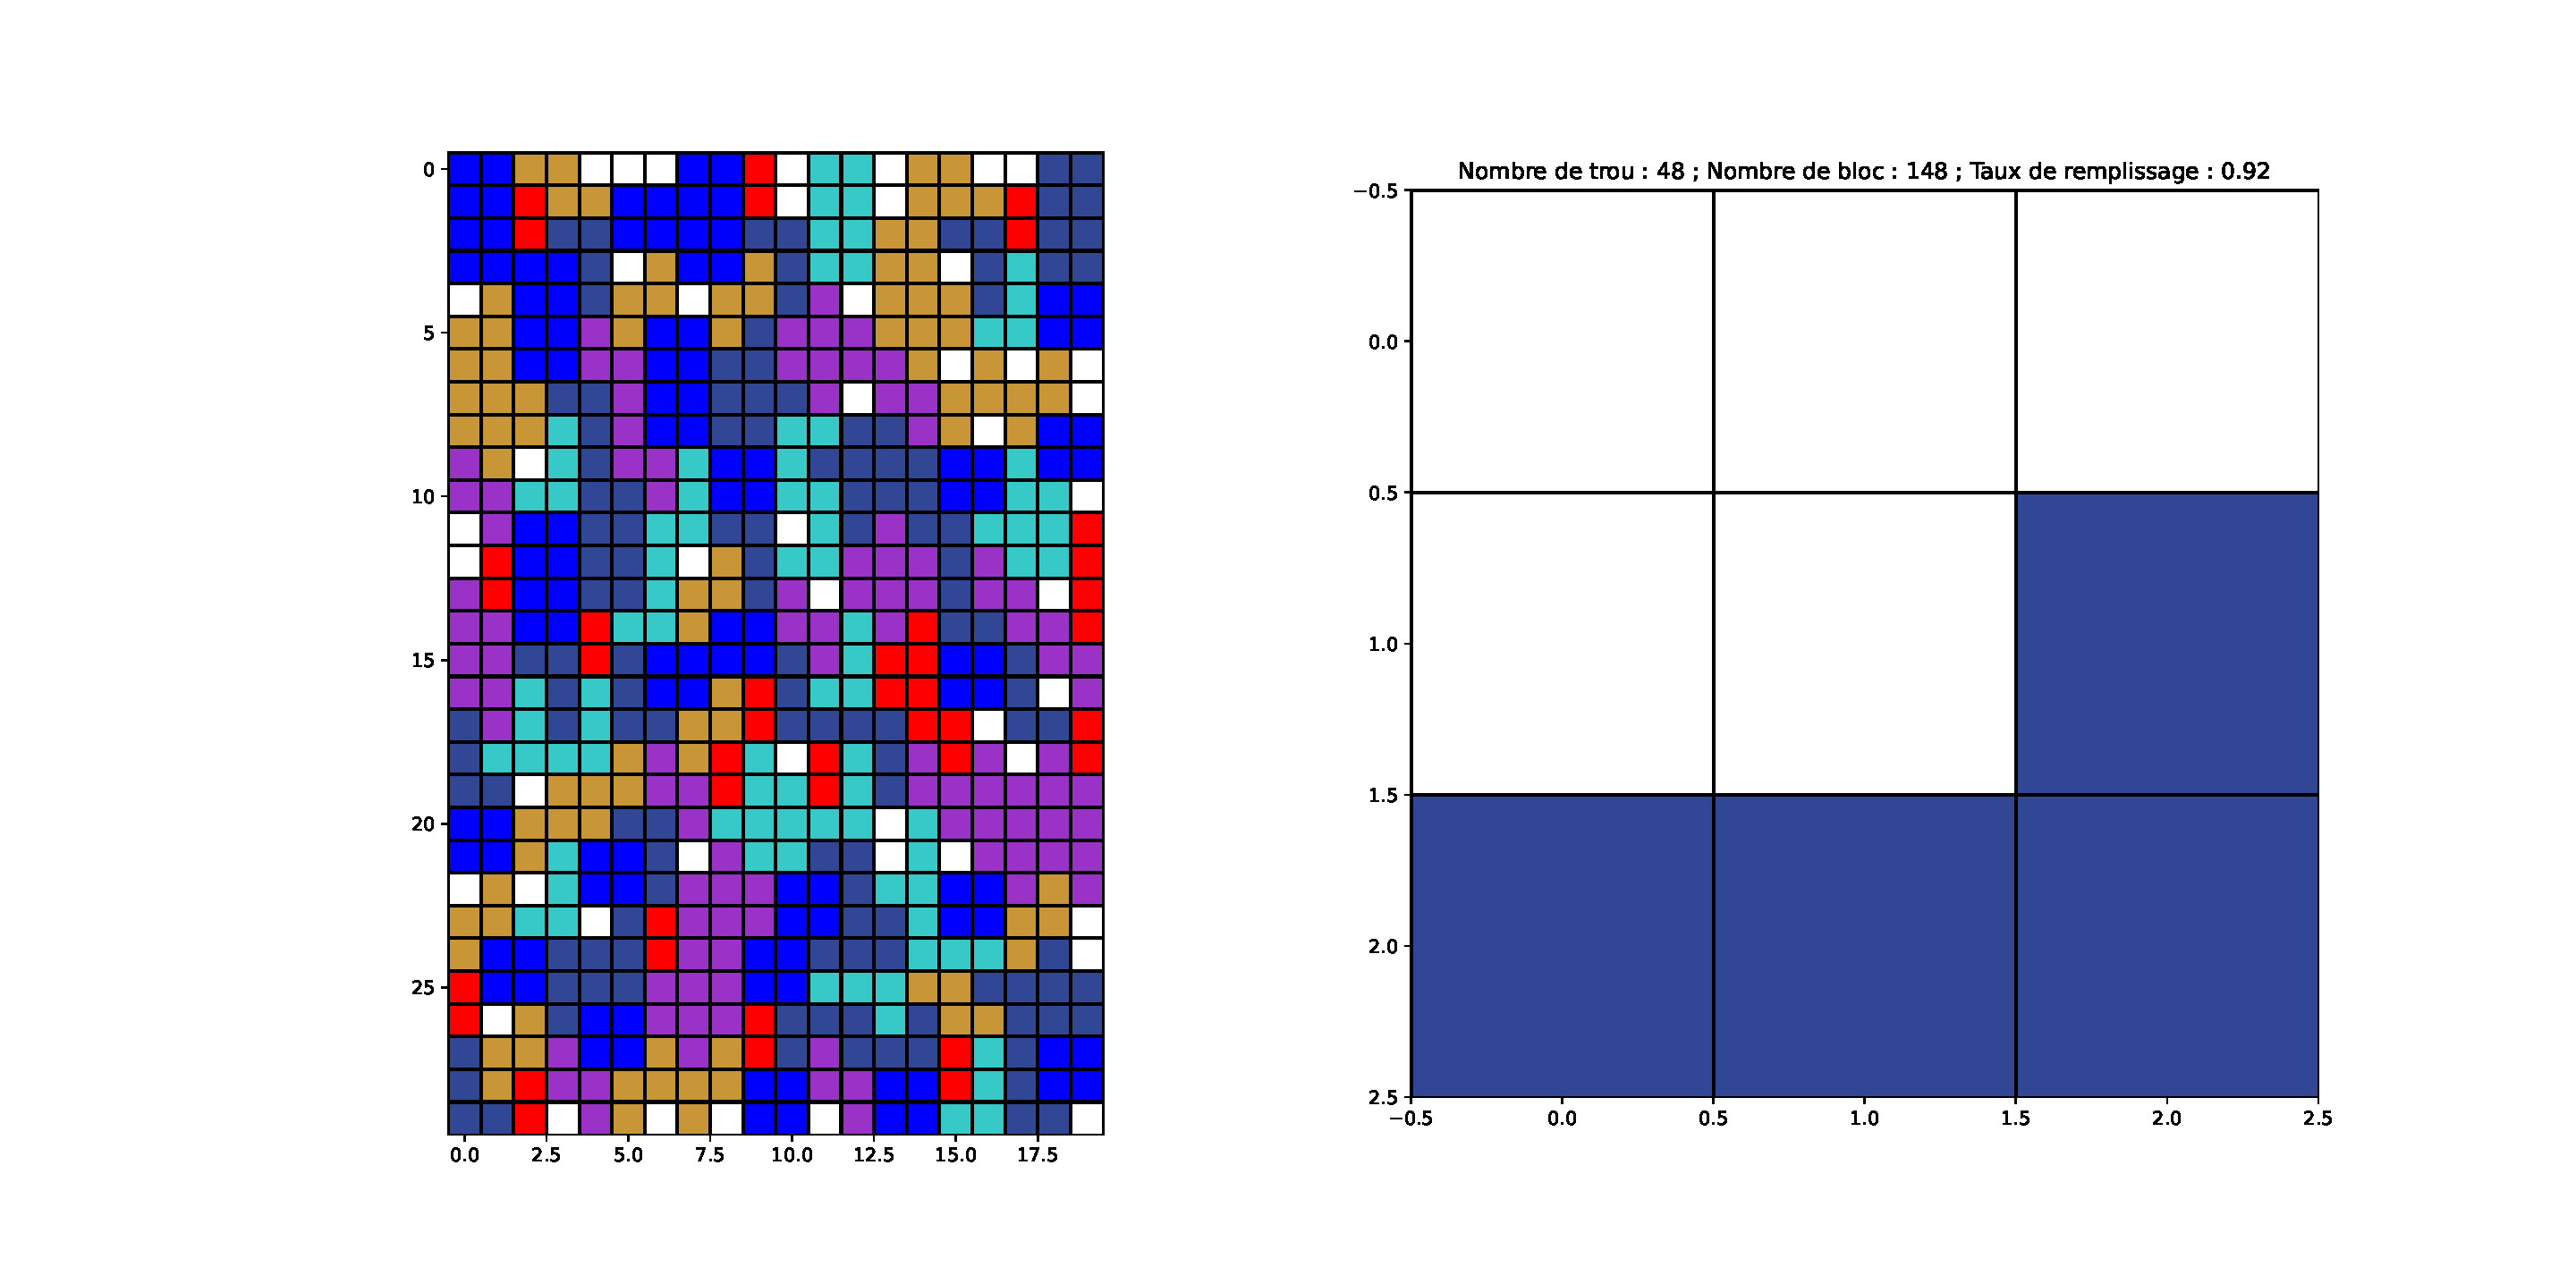
\includegraphics[width=\textwidth]{exemple_grille.pdf}
\end{figure}

\noindent\textbf{Description:}
\begin{itemize}
	\item On dispose d'une grille de taille L$\times$H.
	\item Des blocs tombent dans un premier temps suivant un ordre défini pour que tout le monde puisse se comparer. Ils seront ensuite choisi aléatoirement.
\end{itemize}
\medskip



\noindent\textbf{Objectif:} Proposer un algorithme de décision qui indique la colonne [en partant de la gauche] (et la rotation) dans laquelle placer le bloc pour un état donné de la grille. L'objectif étant de minimiser le nombre de trou dans la grille.

\section*{Déroulement du jeu}

A partir du fichier xxx.py, le jeu se déroule de la façon suivante :

\begin{minted}[bgcolor=bg]{python}
# Initialize game from file
G = set_game_from_file('game_4x4_0.txt')
# Display block list
G.display_all_block_all_config()
# loop until game over
keep_playing = True
while keep_playing:
	s = G.return_game_state()   # get current game state
	a = decision_algo(G, s)     # choose an action
	go = G.update_game_state(a) # update the game
	if go == True:              # check for game over
		print('GAME OVER')
		break

nb_trou, nb_bloc, taux_remplissage = G.print_game_state()
\end{minted}

A partir d'un état du jeu courant \mintinline{python}{s} obtenue par la fonction \mintinline{python}{return_gam_state()}, la fonction \mintinline{python}{decision_algo(G,s)} doit retourner l'action à effectuer pour positionner le bloc nouveau bloc avant de mettre à jour le jeu avec la fonction \mintinline{python}{update_game_state(a)}. Une fois le jeu terminé, la fonction \mintinline{python}{print_game_state()}, en plus d'afficher la grille, renvoie les informations du nombre de trous, du nombres de blocs positionnés et du taux de remplissage dans la grille. 

\subsection*{Travail à faire}

Il s'agit de définir la fonction \mintinline{python}{decision_algo} qui retourne l'action à réaliser pour positionner le bloc courant. Pour cela il est possible de faire appel à la méthode \mintinline{python}{step} de la classe \mintinline{python}{game} qui simule l'état du jeu après avoir positionné le bloc courant avec l'action indiquée:
\begin{minted}[bgcolor=bg]{python}
new_state, game_over = game.step(current_state,action)
\end{minted}

\section*{Quelques explications}

Afin de s'aider dans la prise de décision on dispose de l'état du jeu via la classe \mintinline{python}{state}:

\begin{minted}[bgcolor=bg]{python}
class state:
	# game state 
	# to be used in the decision algorithm
	# return the game state as seen by the 'player' (not all game info are given)
	def __init__(self, grid, b, list_actions):
		self.grid = grid  # H x L matrix
		self.block = b    # block
		self.list_actions = list_actions # list of available action for the current block
\end{minted}

Les informations contenues dans cette classe sont :
\begin{itemize}
	\item La grille est définie par une matrice de taille \mintinline{python}{H}$\times$\mintinline{python}{L}.
	\item Le bloc courant à positionner
	\item La liste de toutes les actions possibles pour le bloc courant.
\end{itemize}
\medskip

Les blocs sont de plusieurs types. Pour afficher tous les blocs possibles vous pouvez utiliser la fonction \mintinline{python}{G.display_all_block_all_config()}.

\begin{figure}[ht!]
	\centering
	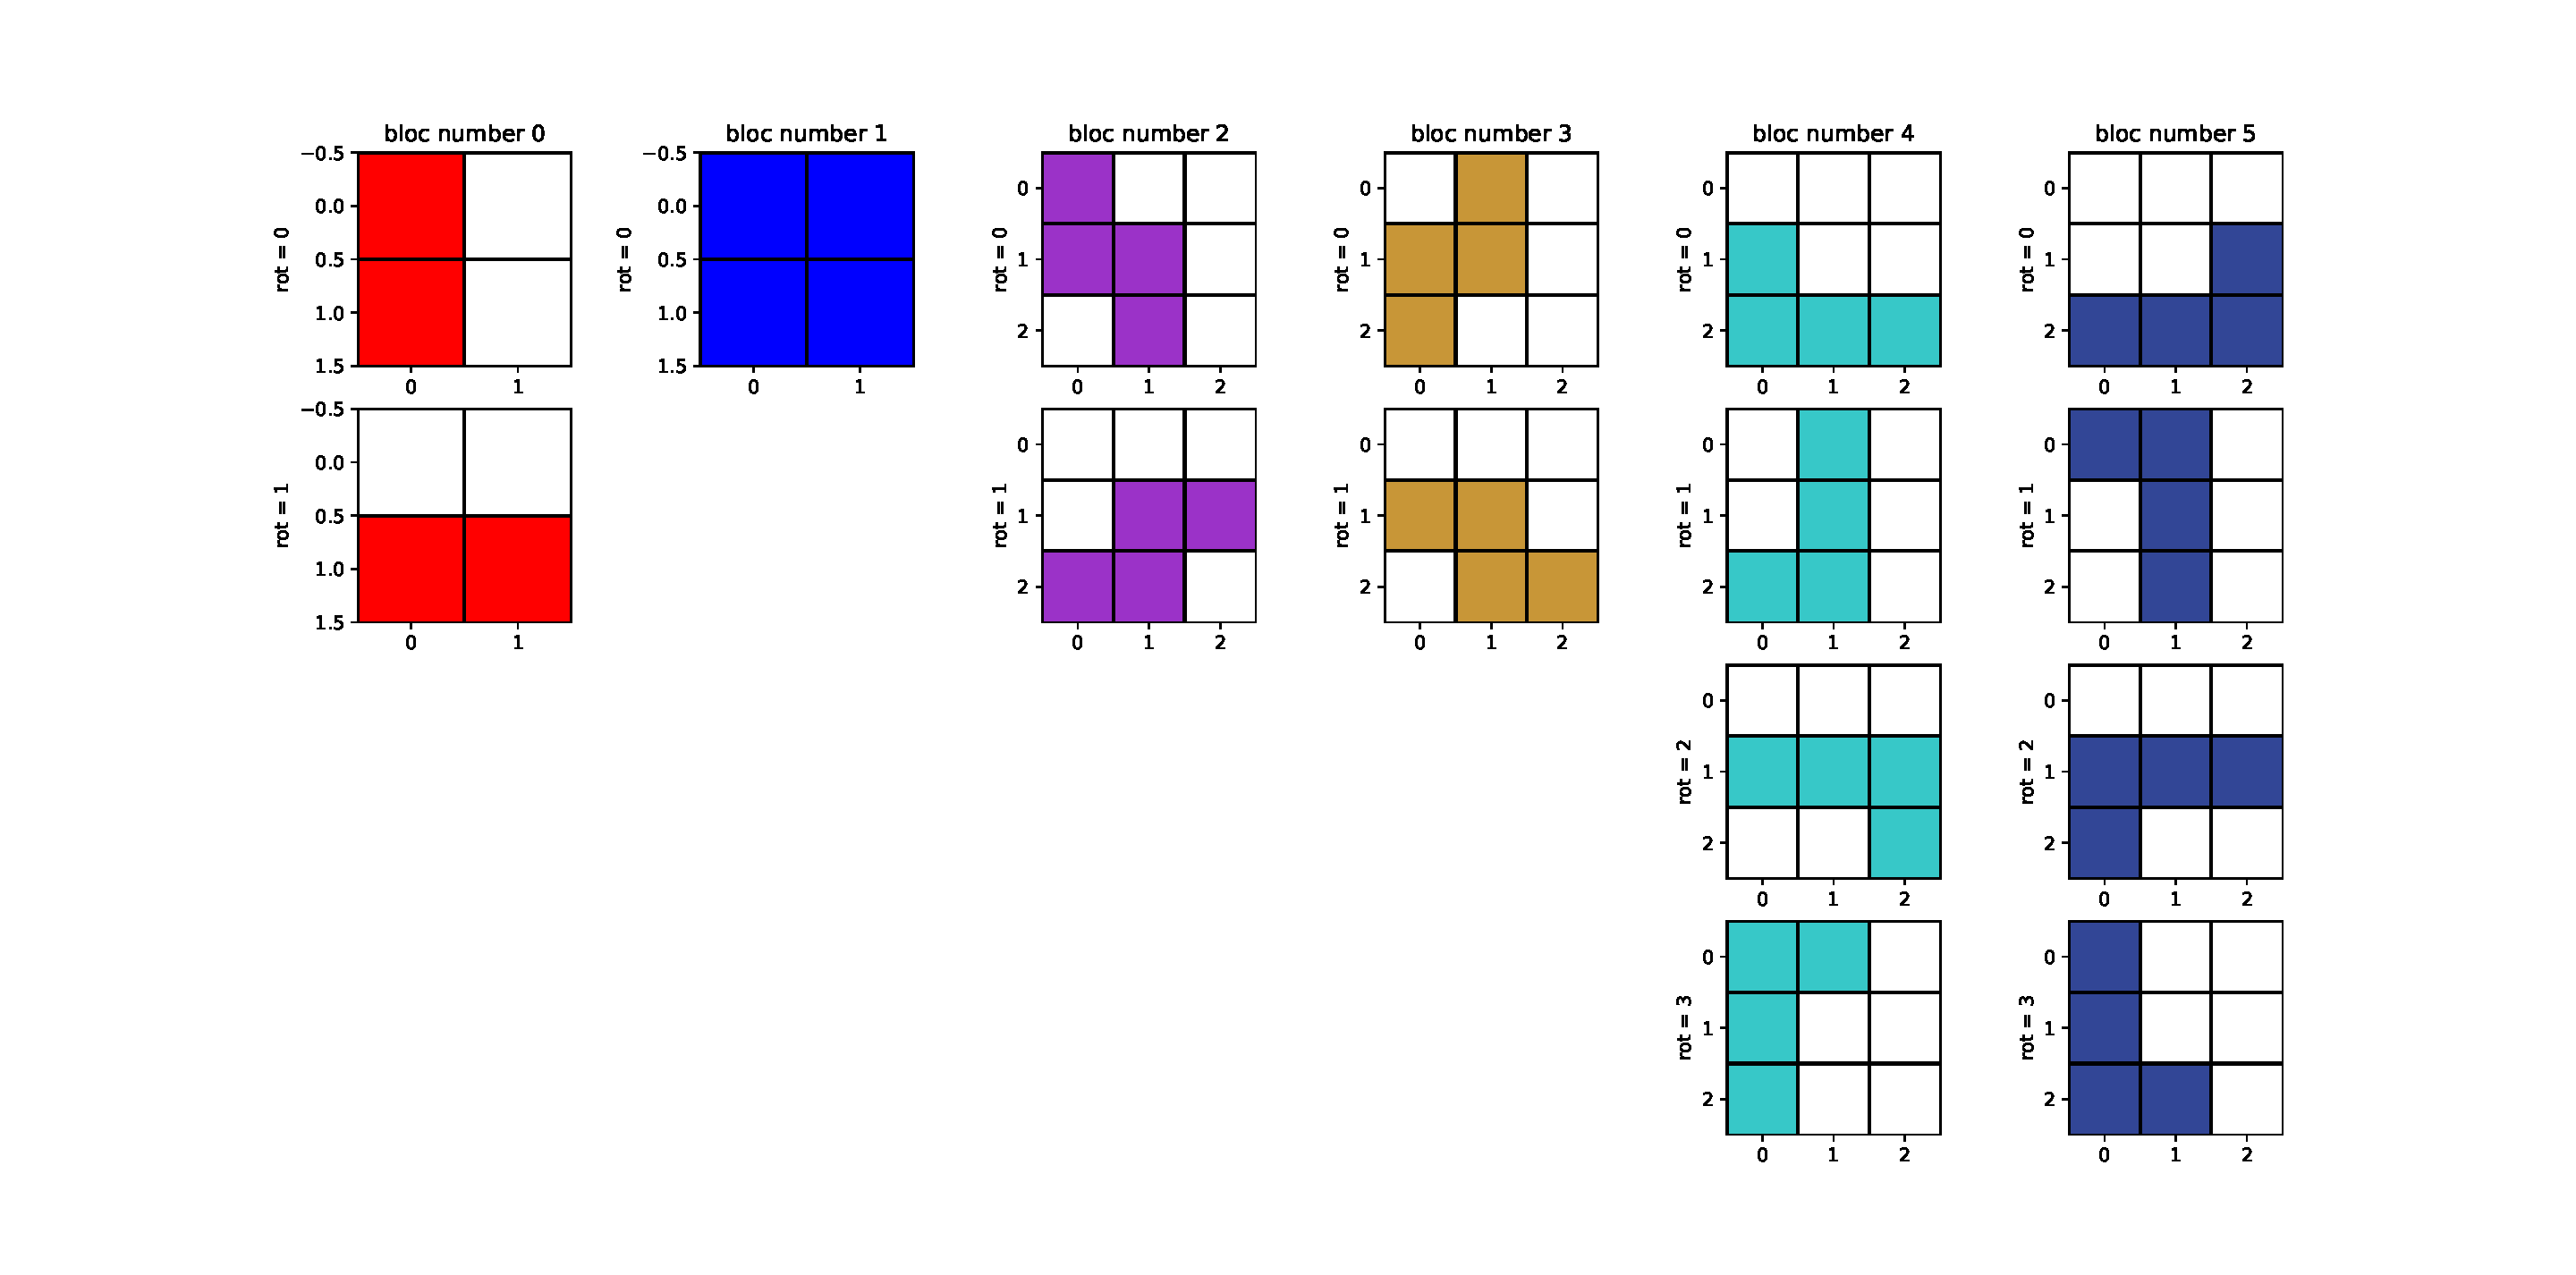
\includegraphics[width=\textwidth]{all_blocks.pdf}
\end{figure}

Chaque bloc est défini par son type, sa valeur dans la grille globale, du nombre de rotation de 90$^o$ possibles et ainsi des différents \mintinline{python}{mask} correspondant à sa forme en fonction de la rotation.
\begin{minted}[bgcolor=bg]{python}
class block:
	# define the different types of blocks
	def __init__(self, type):
		self.mask = []
		if type == 0: # 2x1 block
			self.type = 0   # block type in the game process
			self.value = 1  # value in grid for the block
			self.color = [255, 0, 0]
			self.rot = 2    # number of possible rotations
			self.width = [ 1, 2]
			self.height =[ 2, 1]
			self.mask.append(np.array([[1, 0], [1, 0]]))      
			self.mask.append(np.array([[0, 0], [1, 1]]))      
		elif type == 1: # 2x2 block
\end{minted}

\subsection*{Exemple}

\begin{itemize}
	\item Création d'un nouveau jeu : Ici on considère une grille 10$\times$10 avec un tirage aléatoire des blocs.
\begin{minted}[bgcolor=bg]{python}
G = game(10, 10, fig=True)
G.print_game_state()
\end{minted}

\begin{figure}[ht!]
	\centering
	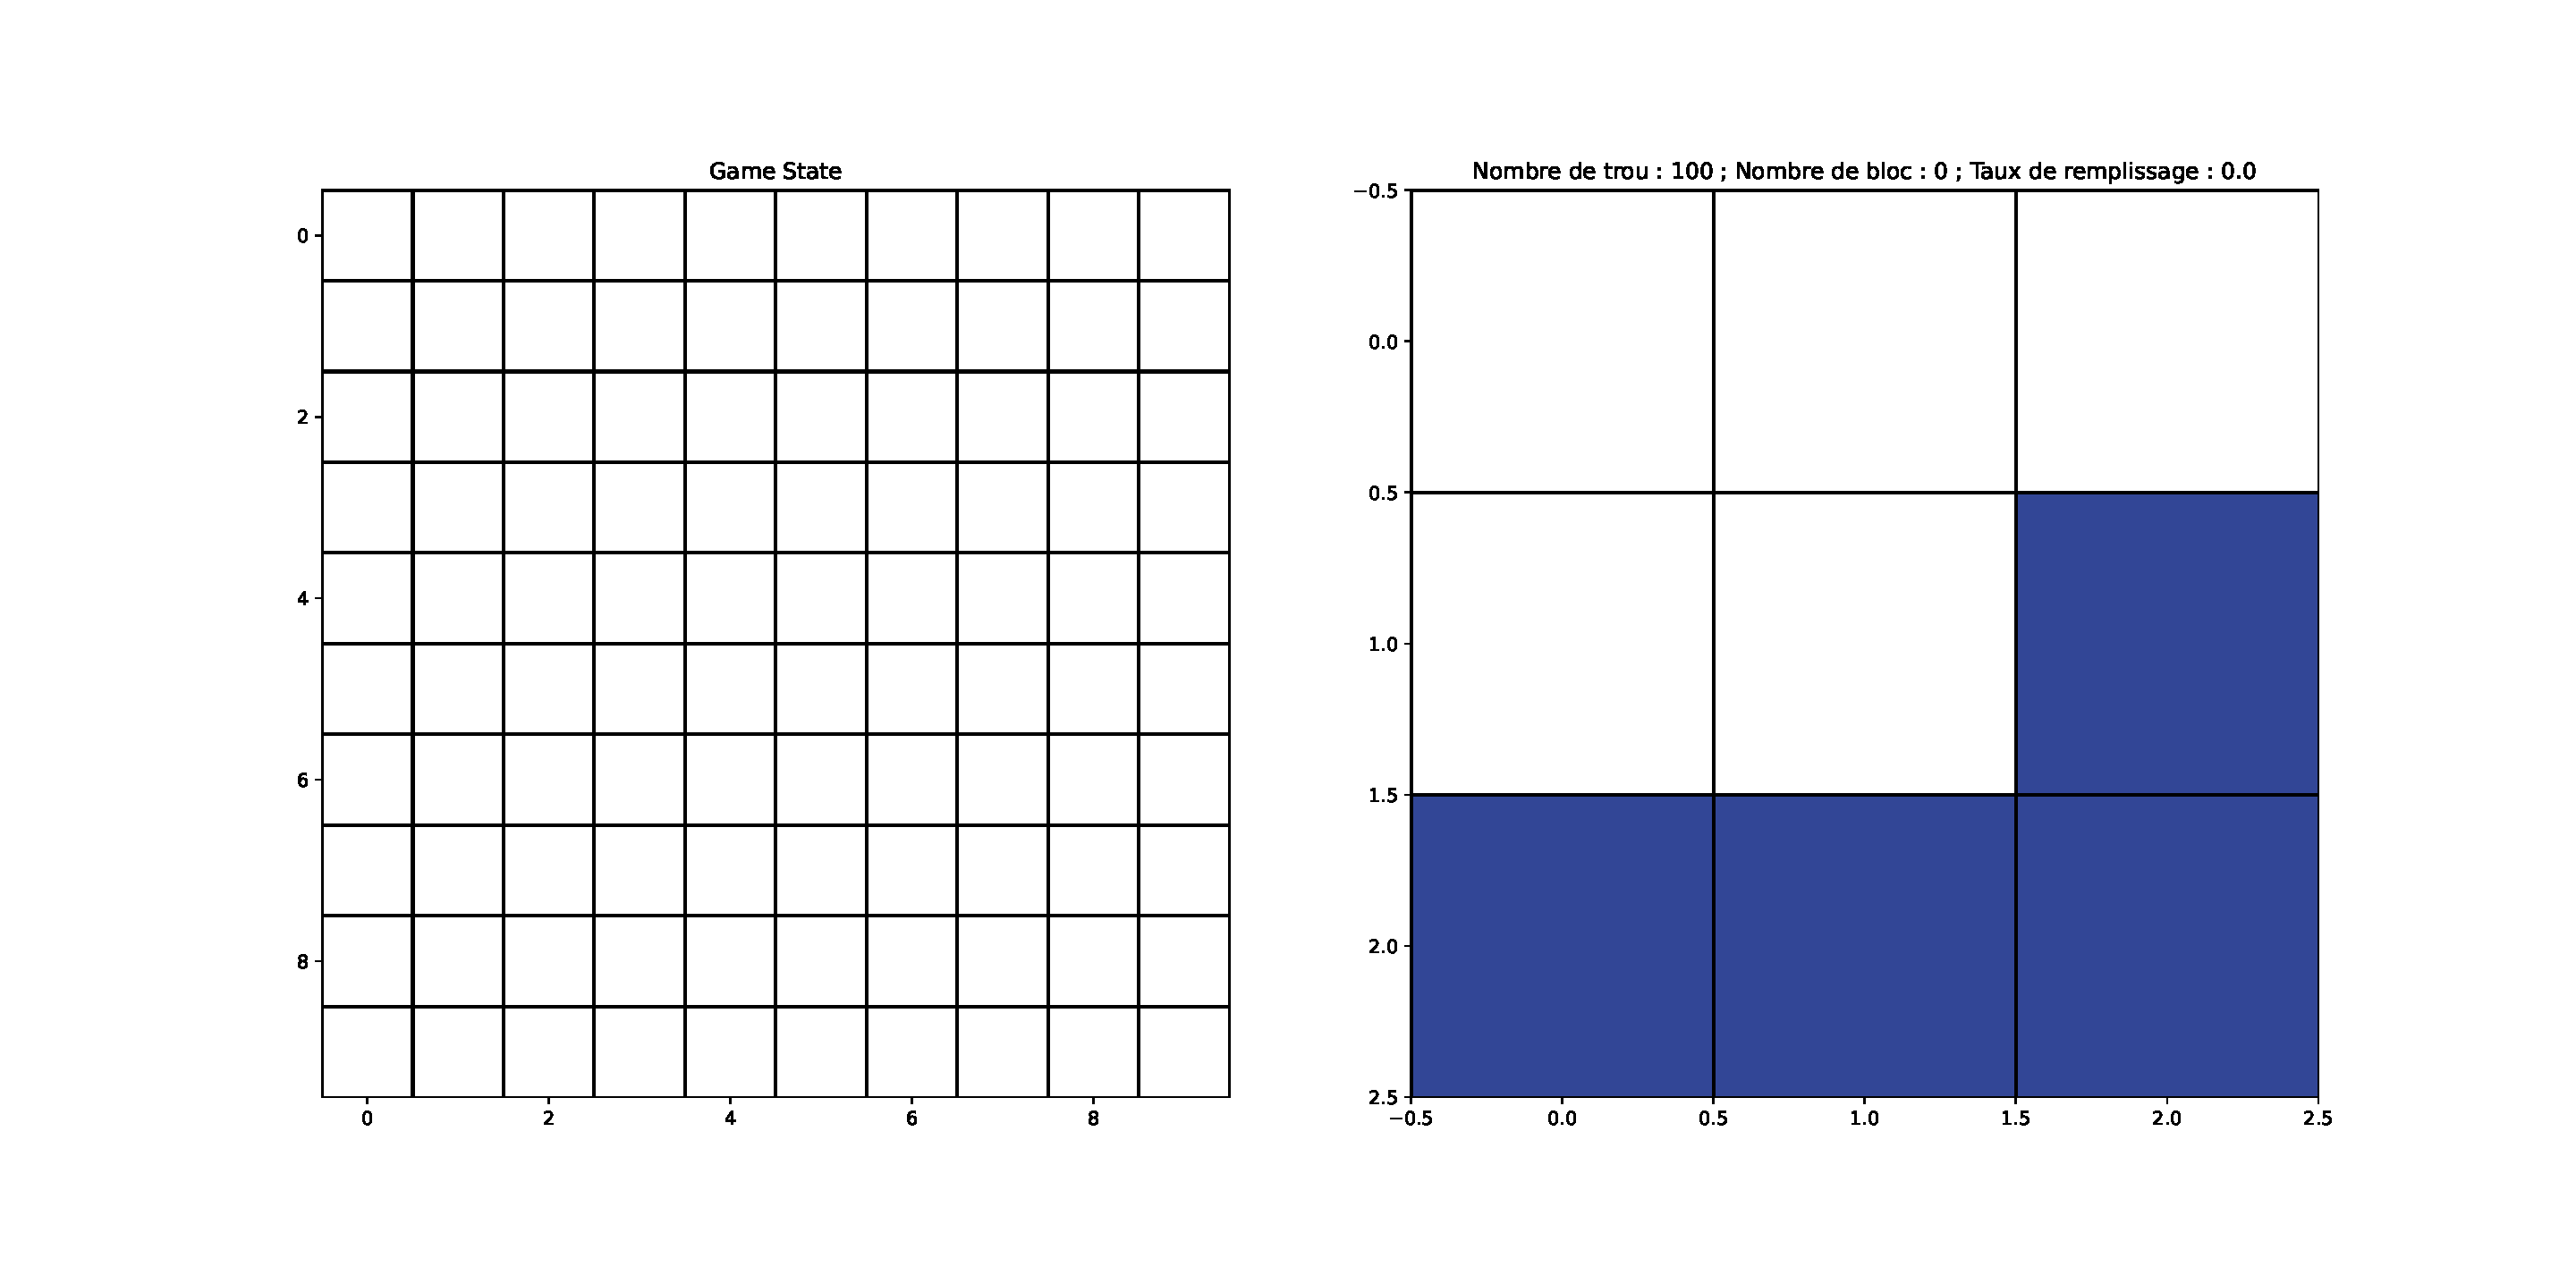
\includegraphics[width=0.7\textwidth]{new_game.pdf}
\end{figure}
\item Positionnement du bloc et mise à jour du jeu.
\begin{minted}[bgcolor=bg]{python}
trans = 1 # numéro de la colonne
rot = 1 # rotation de 90 degrés trigo
ag = action_gene(trans, rot) # classe regroupant les 2 actions
G.update_game_state(ag) # mise à jour du jeu
G.print_game_state()
\end{minted}

On voit apparaître le nouveau bloc à placer à droite.
\begin{figure}[ht!]
	\centering
	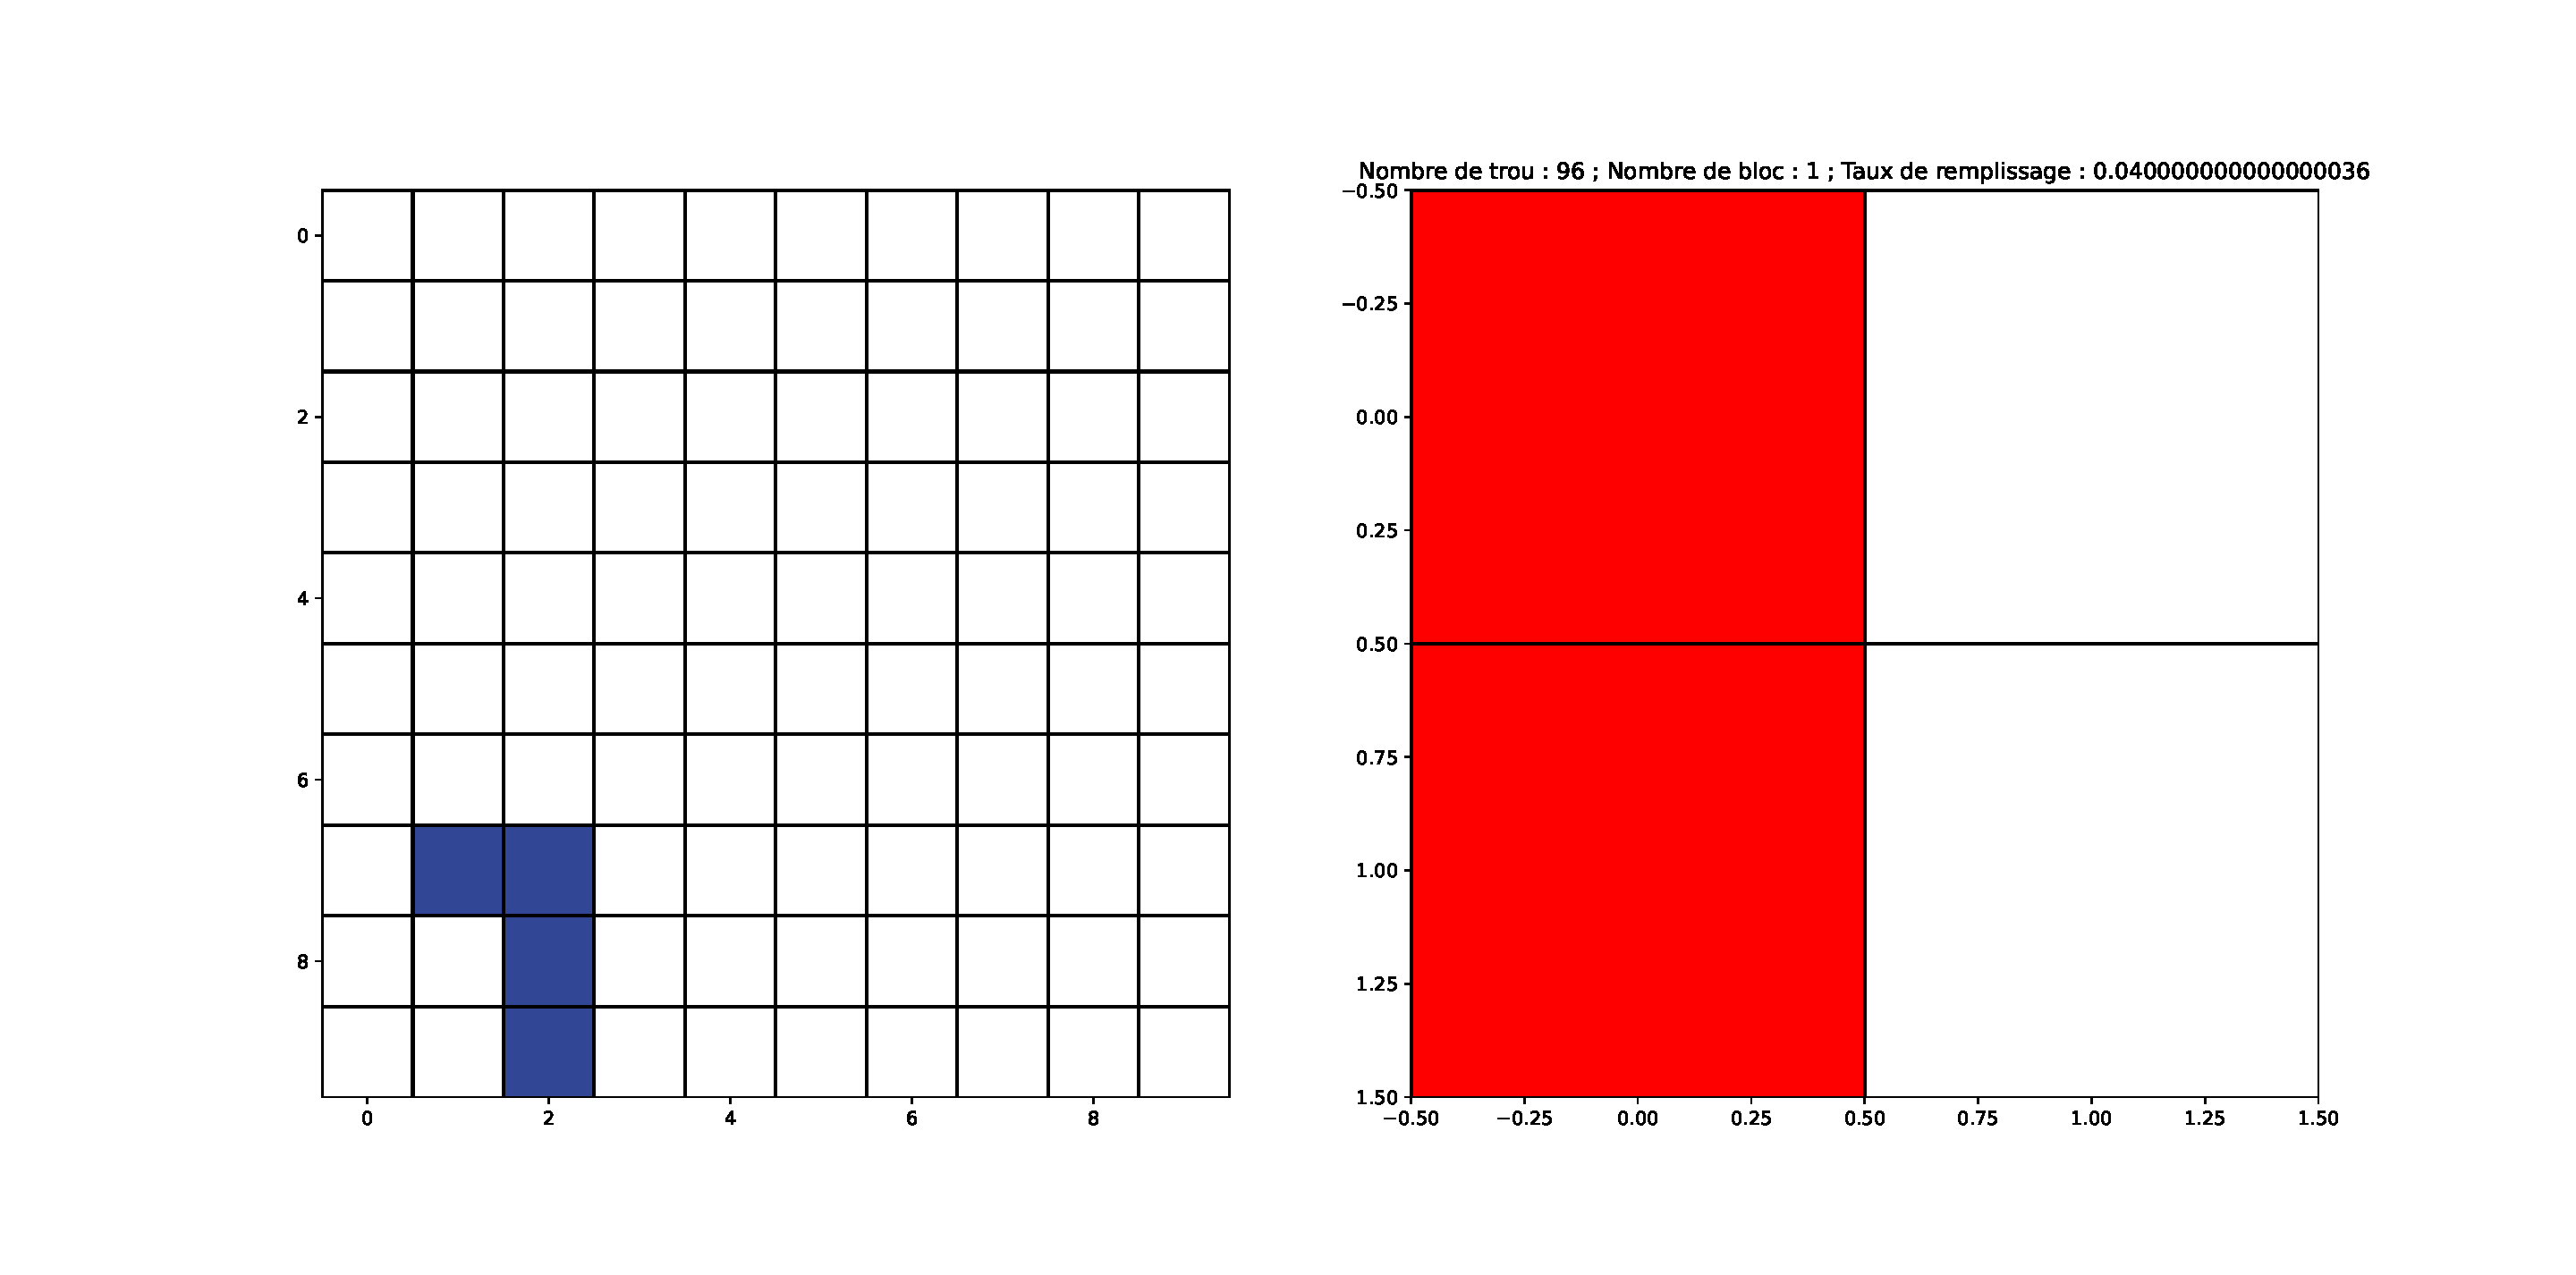
\includegraphics[width=0.7\textwidth]{update_game.pdf}
\end{figure}

\item Positionnement du bloc et mise à jour
\begin{minted}[bgcolor=bg]{python}
trans = 4 # numéro de la colonne
rot = 0 # rotation de 90 degrés trigo
ag = action_gene(trans, rot) # classe regroupant les 2 actions
G.update_game_state(ag) # mise à jour du jeu
G.print_game_state()
\end{minted}
\begin{figure}[ht!]
	\centering
	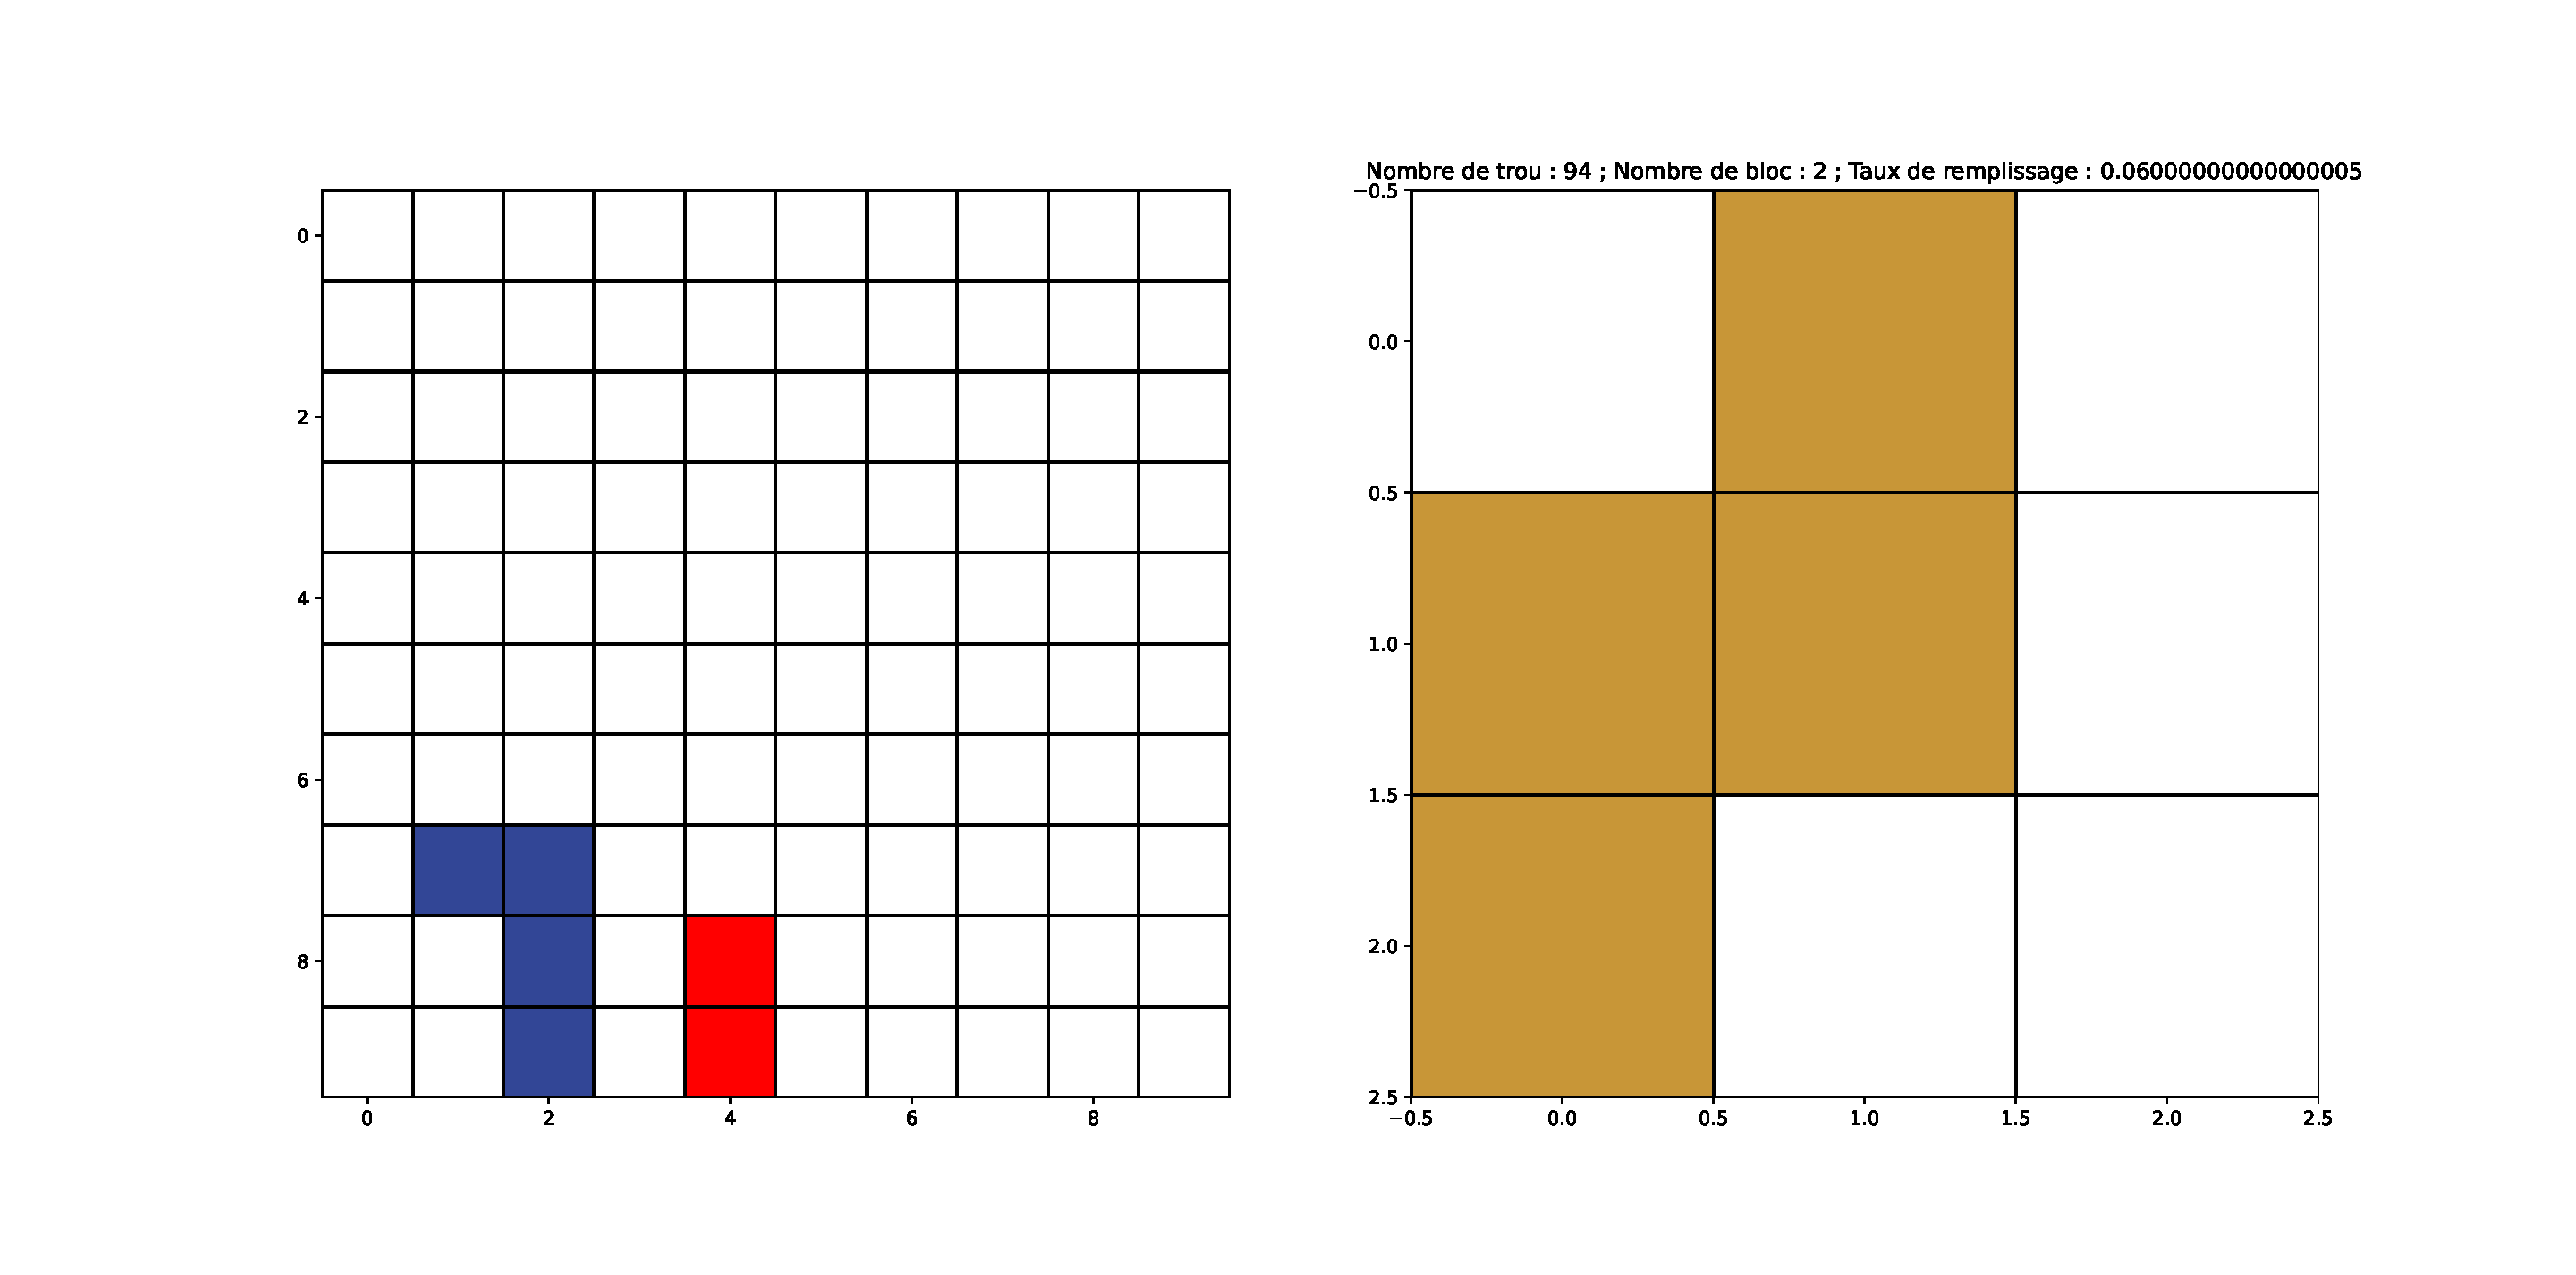
\includegraphics[width=0.7\textwidth]{update_game_2.pdf}
\end{figure}

\end{itemize}

\subsection*{Durant le hackathon}

Afin de tous être confrontés aux mêmes configurations nous vous avons préparer quelques configurations au sein des fichiers \textit{game\_4x4\_0.txt}, \textit{game\_4x4\_1.txt}, \textit{game\_5x5\_0.txt}.

Chacun de ces fichiers est très simple. Par exemple ils comportent les informations de taille de grille ainsi que la liste des blocs qui vont apparaître. Ci-dessous l'exemple du fichier \textit{game\_4x4\_0.txt} qui décrit une taille 4$\times$4 et la liste des numéros des blocs qui apparaîtront durant le jeu.
\begin{minted}[bgcolor=bg]{python}
# Size
4,4
# List of Block
1,0,1,1,0
\end{minted}

\end{document}